%+++++++++++++++++++++++++++++++++++++++++++
\documentclass[conference]{IEEEtran}
%+++++++++++++++++++++++++++++++++++++++++++
% Added to commands
\input epsf
\usepackage{graphicx}
\usepackage{url}
\usepackage{subcaption}

%+++++++++++++++++++++++++++++++++++++++++++
% correct bad hyphenation here
\hyphenation{op-tical net-works semi-conduc-tor IEEEtran}
\begin{document}

%+++++++++++++++++++++++++++++++++++++++++++
% paper title
\title{\LARGE Network Analysis of 'MiBici' Public Bike Service in Guadalajara's Metropolitan Area}

\author{Henry Marie MONT and Matteo MATONE \\
University of Tartu, Department of Computer Science \\
Tartu, Estonia \\
\texttt{henry.marie.mont@ut.ee, matone@ut.ee}}

\maketitle

\begin{abstract}

% This paper presents a comprehensive network analysis of the public shared bike service known as "MiBici" in Guadalajara's metropolitan area (ZMG) in Jalisco, Mexico, spanning from December 2014 to January 2024. We explore the network structure, dynamics, and user behaviors of the "MiBici" system using different network analysis techniques. Through data preprocessing, network construction, and analysis scripts, we uncover insights into the spatial distribution of bike stations, traffic flows, user mobility patterns, and system efficiency. Our findings contribute to enhancing the understanding of public bike-sharing systems and provide valuable insights for urban planning and transportation management.

WORK IN PROGRESS

\end{abstract}
\IEEEoverridecommandlockouts
\begin{keywords}
% Public bike-sharing, Network analysis, Complex network theory, Urban transportation, Mexico, Guadalajara.

WORK IN PROGRESS
\end{keywords}

\section{Introduction}

% Public bike-sharing systems have become increasingly popular in urban areas as a sustainable and convenient mode of transportation. These systems provide users with access to bicycles for short trips, contributing to reducing traffic congestion and promoting healthier lifestyles. Understanding the dynamics of public bike-sharing systems, including network structure, user behaviors, and system efficiency, is crucial for optimizing service operations and guiding urban planning efforts.

% In this paper, we focus on the network analysis of the "MiBici" public bike service in Guadalajara's metropolitan area (ZMG) in Jalisco, Mexico. By exploring the spatial distribution of bike stations, traffic flows, and user mobility patterns, we aim to gain insights into the functioning of the "MiBici" system and its implications for urban transportation in Guadalajara.

WORK IN PROGRESS

\section{Related work}

The exploration of public bicycle systems through network analysis has garnered significant attention in recent literature, offering insights into system structure, dynamics, and user behaviors. Wei, Xu, and Ma \cite{wei2019exploring} demonstrated the applicability of complex network theory and shortest path analysis in characterizing the public bicycle network structure in Yixing, China. Yao et al. \cite{yao2019analysis} focused on analyzing urban bike-sharing systems using real-time data from the Nanjing public bicycle system. Dobrzyńska and Dobrzyński \cite{dobrzynska2017structure} conducted a comprehensive analysis of the BiKeR public bike-sharing system in Białystok, Poland, emphasizing the dynamics of network topology changes and station location choices. Jurdak \cite{jurdak2013impact} investigated the impact of cost and network topology on urban mobility using data from public bicycle share systems in two U.S. cities. Xiao et al. \cite{xiao2021demand} addressed the challenge of short-term demand prediction in public bike-sharing programs, proposing a spatio-temporal graph convolutional network (STGCN) approach. Builes-Jaramillo and Lotero \cite{builes-jaramillo2022spatial} conducted spatial-temporal network analysis of the public bicycle sharing system in Medellín, Colombia. 

These studies collectively contribute to advancing knowledge on public bicycle systems, offering insights into network structure, dynamics, user behaviors, and planning strategies, which are instrumental in promoting sustainable urban transportation.

\section{Dataset}

\subsection{Source}
The dataset used in this analysis is a public dataset from Kaggle, specifically sourced from the MiBici public bike service in Guadalajara's metropolitan area (ZMG) in Jalisco, Mexico. It spans from December 2014 to January 2024, covering 110 months in total. The dataset comprises 25,863,690 public bike trips and includes information on 372 public bike stations \cite{quirarte2024mibici}.

\subsection{Data Description}
The dataset comprises two main components: the Nomenclature dataset and the MiBici dataset. The Nomenclature dataset consists of 372 entries, providing information about bike station locations within the Guadalajara Metropolitan Area. Each entry includes details such as station ID, name, location, latitude, longitude, and status. The MiBici dataset contains 25,863,690 entries and records bike trip information spanning from 2014 to 2024. It includes trip IDs, user IDs, demographics (sex, birth year), trip start and end times, origin and destination station IDs, user age, and trip duration.

\subsection{Data Preprocessing}
The raw dataset was pruned to improve efficiency due to its large size, reducing it to approximately 1/10th of its original size. The pruned dataset was then exported to a CSV file named 'mibici\_compact.csv' that you will be able to find on our github page.

Stations marked as 'NOT\_IN\_SERVICE' were removed from the 'nomenclature' dataset to ensure that only active stations were included. Additionally, columns such as 'obcn', 'location', and 'status' were dropped from the 'nomenclature' dataset as they were deemed unnecessary for the analysis.

In the pruned 'MiBici' dataset, datetime columns ('Trip\_start' and 'Trip\_end') were converted to datetime objects to facilitate temporal analysis. The 'Duration' column, representing the duration of each bike trip, was converted to numerical format (seconds) for easier computation. Additional features, such as 'Day\_of\_week', 'Hour\_of\_day', and 'Month', were extracted from the datetime columns to provide more granular insights into temporal patterns. Finally, unnecessary columns such as 'Unnamed: 0', 'User\_Id', 'Sex', 'Birth\_year', and 'Age' were dropped from the pruned 'MiBici' dataset to streamline further analysis (those will be reinserted later on for prediction algorithms purposes if times allow it).

\subsection{Constructing the Network}
The network was constructed by creating a directed and weighted graph to represent the 'MiBici' public bike service in Guadalajara. Nodes, corresponding to bike stations, were added using data from the 'nomenclature' dataset, including station ID, name, latitude, and longitude. Edges representing bike trips between stations were derived from the pruned 'MiBici' dataset. For each trip record, if an edge didn't exist already, it was created. Otherwise the edge weight was incremented to reflect the number of trips between stations. To facilitate analysis and identify patterns, graphs could be generated based on specific criteria such as years or days of the week later on. The network graph was visualized with nodes positioned according to geographical coordinates to illustrate the spatial layout of bike stations and trip connections (see Figure \ref{fig:side_by_side}).

\begin{figure}[htbp]
    \centering
    \begin{subfigure}[b]{0.20\textwidth}
        \centering
        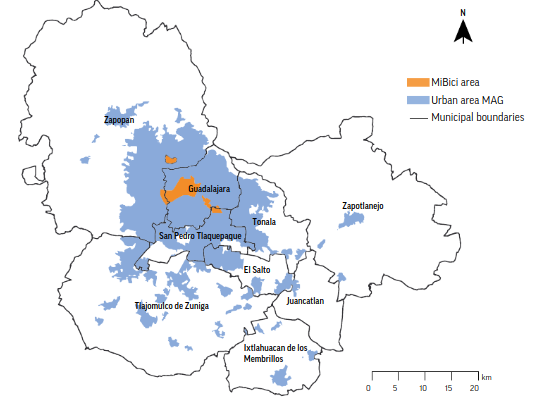
\includegraphics[width=\textwidth]{images/urban-areas-covered-mibici.png}
        \caption{Map of the MiBici network}
        \label{fig:network}
    \end{subfigure}
    \hfill
    \begin{subfigure}[b]{0.20\textwidth}
        \centering
        \includegraphics[width=\textwidth]{images/mibici-network.png}
        \caption{Constructed network}
        \label{fig:map}
    \end{subfigure}
    \caption{Real network vs our network}
    \label{fig:side_by_side}
\end{figure}

\subsection{Descriptive Analysis of the network}

The network comprises 359 nodes representing various entities interconnected by 37,031 edges, reflecting relationships between these entities. This network is directed and weighted. With an average path length of around 1.81, the network reveals numerous lightly utilized pathways between bike stations, contributing to the slightly lower average path length. A single large connected component signifies that all parts of the bike network are interconnected, ensuring comprehensive coverage across the city. However, with a density of approximately 0.29, only about 29\% of all possible connections exist, implying that certain rides between specific stations are infrequent. This aligns with the logical expectation that riding between very close or distant stations may be less common. The high reciprocity, nearing 0.78, indicates a substantial number of mutual connections between nodes, likely reflecting regular commuting patterns such as travel to work or school. Furthermore, the clustering coefficient, approximately 0.68, suggests a tendency for nodes to cluster together, reflecting typical travel patterns where people frequently move between specific areas, creating traffic clusters, such as between city centers and residential zones.

\section{Methodology}

\subsection{Literature Review and Exploratory Data Analysis}
The study will commence with a comprehensive literature review to comprehend the existing research landscape and to identify relevant features and patterns in the domain of interest. Concurrently, exploratory data analysis (EDA) will be conducted on the available dataset to gain insights into its structure, distribution, and potential relationships between variables.

\subsection{Data Preprocessing}
Following EDA, data preprocessing will be performed to prepare the dataset for further analysis. This step will involve cleaning the data, handling missing values, and standardizing formats to ensure consistency and accuracy. Additionally, the dataset will be pruned to a tenth of its original size to facilitate efficient processing.

\subsection{Feature Selection}
Based on insights gained from the literature review and EDA, relevant features will be selected for analysis. Features will be chosen based on their potential to contribute meaningful information to the study objectives. Information such as stations' names and coordinates, trips' origin, destination, datetime, and duration will be retained.

\subsection{Graph Construction}
Using the selected features, a graph representation of the data will be constructed. Each bike station in the dataset will be represented as a node, and trips between stations will be represented as edges. The graph will provide a structured framework for analyzing relationships and patterns within the dataset.

\subsection{Exploratory Analysis of Graph}
Basic descriptive analysis will be conducted on the constructed graph to gain a better understanding of its properties. Information such as average path length, density, and reciprocity will be computed to inform further analysis.

\subsection{Network Preprocessing}
To ensure the integrity of the network analysis, preprocessing steps such as removing disconnected nodes or nodes with low edge connections will be performed. This step will help streamline the analysis and focus on meaningful network structures.

\subsection{Pattern Identification}
Using exploratory techniques, interesting patterns within the network data will be identified. These patterns could include trends such as hourly, daily, or monthly variations, as well as differences between weekdays and weekends. Specific visualizations will be created to explore and analyze these patterns effectively.

\subsection{Network Property Analysis}
For identified patterns, key network properties and metrics will be analyzed to understand their underlying characteristics and dynamics. This analysis will provide insights into the structural properties of the network and how they evolve over time.

\subsection{Result Interpretation}
Finally, the results of the analysis will be interpreted, drawing conclusions and implications based on the observed patterns and network properties. This step will involve synthesizing findings from multiple analyses to provide a comprehensive understanding of the dataset and its underlying dynamics.

\begin{figure}
    \centering
    \includegraphics[width=0.75\linewidth]{images/Flowchart.png}
    \caption{Network analysis flowchart}
    \label{fig:flowchart}
\end{figure}

\section{Results}

WORK IN PROGRESS

\section{Conclusion}

WORK IN PROGRESS

\begin{thebibliography}{1}

\bibitem{wei2019exploring}
Wei, Sheng, Jiangang Xu, and Haitao Ma. “Exploring Public Bicycle Network Structure Based on Complex Network Theory and Shortest Path Analysis: The Public Bicycle System in Yixing, China.” \textit{Transportation Planning and Technology} 42, no. 3 (2019): 293–307. doi:10.1080/03081060.2019.1576385.

\bibitem{yao2019analysis}
Yao, Yi, Yifang Zhang, Lixin Tian, Nianxing Zhou, Zhilin Li, and Minggang Wang. 2019. "Analysis of Network Structure of Urban Bike-Sharing System: A Case Study Based on Real-Time Data of a Public Bicycle System" \textit{Sustainability} 11, no. 19: 5425. https://doi.org/10.3390/su11195425.

\bibitem{dobrzynska2017structure}
Dobrzyńska, Ewa, and Dobrzyński, Maciej. "Structure and dynamics of a public bike-sharing system. Case study of the public transport system in Białystok" \textit{Engineering Management in Production and Services} 8, no.4 (2017): 59-66. https://doi.org/10.1515/emj-2016-0033.

\bibitem{jurdak2013impact}
Jurdak, Raja. "The Impact of Cost and Network Topology on Urban Mobility: A Study of Public Bicycle Usage in 2 U.S. Cities." \textit{PLoS ONE} 8, no. 11 (2013): e79396. https://doi.org/10.1371/journal.pone.0079396.

\bibitem{xiao2021demand}
Xiao, G., Wang, R., Zhang, C. et al. Demand prediction for a public bike sharing program based on spatio-temporal graph convolutional networks. \textit{Multimed Tools Appl} 80, 22907–22925 (2021). https://doi.org/10.1007/s11042-020-08803-y.

\bibitem{builes-jaramillo2022spatial}
Builes-Jaramillo, Alejandro, and Laura Lotero. "Spatial-temporal network analysis of the public bicycle sharing system in Medellín, Colombia." \textit{Journal of Transport Geography} 105 (2022): 103460. https://doi.org/10.1016/j.jtrangeo.2022.103460.

\bibitem{torres2021sustainable}
Torres, Arturo, Ortega, Andrea, Sudmant, Andrew, \& Gouldson, Andy. (2021). Sustainable Mobility for Sustainable Cities: Lessons from Cycling Schemes in Mexico City and Guadalajara, Mexico.

\bibitem{quirarte2024mibici}
Quirarte, Sebastián. (2024). Over 9 Years of Real Public Bike Use Data - MiBici. Kaggle. \url{https://www.kaggle.com/datasets/sebastianquirarte/over-9-years-of-real-public-bike-use-data-mibici}

\end{thebibliography}

\section{Github}

The source code of the project can be viewed on Github at \url{https://github.com/monthenry/Network-Science-Project}.

\end{document}